\chapter{Metodologia de medição}
\mbox{}

Para desenvolver o estudo empírico deste trabalho, precisamos de meios para medir a energia consumida por aplicações. Neste pequeno capítulo, primeiro apresentamos a máquina com o sistema que permite medir seu consumo energético, e depois explicamos como tratamos estes dados para obter o consumo de aplicações.

\section{Sobre o sistema utilizado}
\mbox{}

O sistema utilizado foi gentilmente emprestado pelo Professor Hermes Senger, da Universidade Federal de São Carlos, e seu grupo. Tal sistema é composto por uma máquina, à que nos foi concedido o acesso por SSH, cuja fonte de alimentação é ligada a um sensor de potência que envia os valores para o servidor de dados MW100 Yokogawa. A taxa máxima de amostragem que conseguimos é de 2 valores a cada segundo.

Terminais sob a rede da UFSCar podem requerer dados do MW100 por duas interfaces: Web e Telnet. O MW100 também oferece, ao administrador, a possibilidade de gravar os valores durante certo intervalo. Porém, como nosso acesso é restrito, escrevemos uma simples biblioteca estática para encapsular as requisições Telnet e permitir que gravássemos os dados para análise futura.

\begin{figure}[htp]
\centering
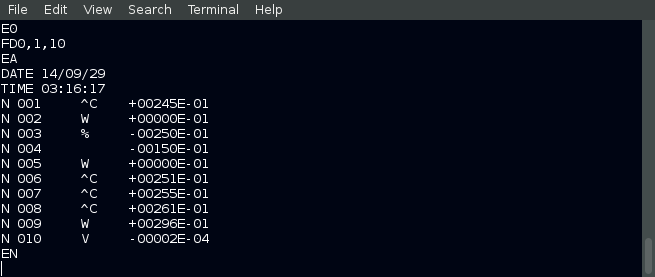
\includegraphics[scale=0.5]{figuras/MetMed/MW100telnet.png}
\caption{Acesso por Telnet}
\label{MW100telnet}
\end{figure}

A máquina de testes possui as seguintes configurações:

\begin{itemize}
    \item RAM: 4GB
    \item CPU: Intel Core i5-2400 @ 3.1Ghz
    \item SO: Ubuntu (kernel 3.2.0) 64 bits
\end{itemize}

\section{Gravando o consumo de potência}
\mbox{}

Como foi dito, não temos o direito de requerer gravações ao sistema MW100. Assim, escrevemos a biblioteca estática\footnote{Note que esta biblioteca está muito longe de ser o foco do trabalho e foi escrita apenas por problemas de acesso. Assim, este capítulo não traz nada parecido com uma documentação, apenas simples descrições para que o leitor possa entender melhor nosso sistema de medição.} {\tt mw100\_recorder} que oferece ao usuário comum a possibilidade de utilizar a própria máquina para fazer requisições de última medição e gravar os valores lidos.

%Obviamente, ao utilizar a mesma máquina para executar aplicações e fazer requisições para o servidor, o consumo total é afetado. Porém....

A interface que a biblioteca oferece é a seguinte:

\begin{lstlisting}[language=C, basicstyle=\ttfamily\footnotesize, frame=single]
void mw100_recorder_init(char mw100ip4[], int mw100port, 
                         double time_interval, int channel);
void mw100_recorder_start(int verbose);
void mw100_recorder_stop(int verbose);
void mw100_get_recorded_info(mw100_record_info *p_user_info);
\end{lstlisting}

O funcionamento da biblioteca é extremamente simples como pode ser visto pela descrição, em alto nível, de cada função:

\begin{itemize}
\item {\tt void mw100\_recorder\_init()}:

Inicializa o gravador passando como parâmetros o IP do servidor MW100, a porta sob a qual roda o Telnet, o intervalo aproximado de tempo entre requisições, e o canal do MW100 a que está conectado o sensor de potência.

\item {\tt void mw100\_recorder\_start()}:

Começa uma gravação e, dependendo do parâmetro passado, imprime os valores na saída padrão. A gravação é feita através de um \emph{thread} criado especificamente para fazer requisições e gravar os valores lidos.

\item {\tt void mw100\_recorder\_stop()}:

Finaliza uma gravação, terminando o \emph{thread} que havia sido criado.


\item {\tt void mw100\_get\_recorded\_info()}:

Sobrescreve os valores do elemento passado por referência com os da medição que acabou de ser feita. Na estrutura de dados específica para conter estas informações, temos os dados de potência média, energia total consumida e tempo total de medição.

\end{itemize}

Para testar a biblioteca, desenvolvemos uma ferramenta chamada {\tt powerdump} que, passados um intervalo de tempo em segundos e um arquivo, usa a biblioteca para obter os valores de potência e escrevê-los no arquivo passado. 

Utilizando esta ferramenta, determinamos os picos de consumo da máquina, executamos o seguinte:
\begin{itemize}
\item Para $ n = 1, 2, ..., 8 $, faça:
 \begin{itemize}
  \item espere 10 segundos
  \item rode, paralelamente, $ n $ processos que calculam as 30.000 casas decimais de $ \pi $
 \end{itemize}
\end{itemize}

Os valores obtidos nesta gravação podem ser vistos na Figura \ref{powerdump_pidigits}.

\begin{figure}[htp]
\centering
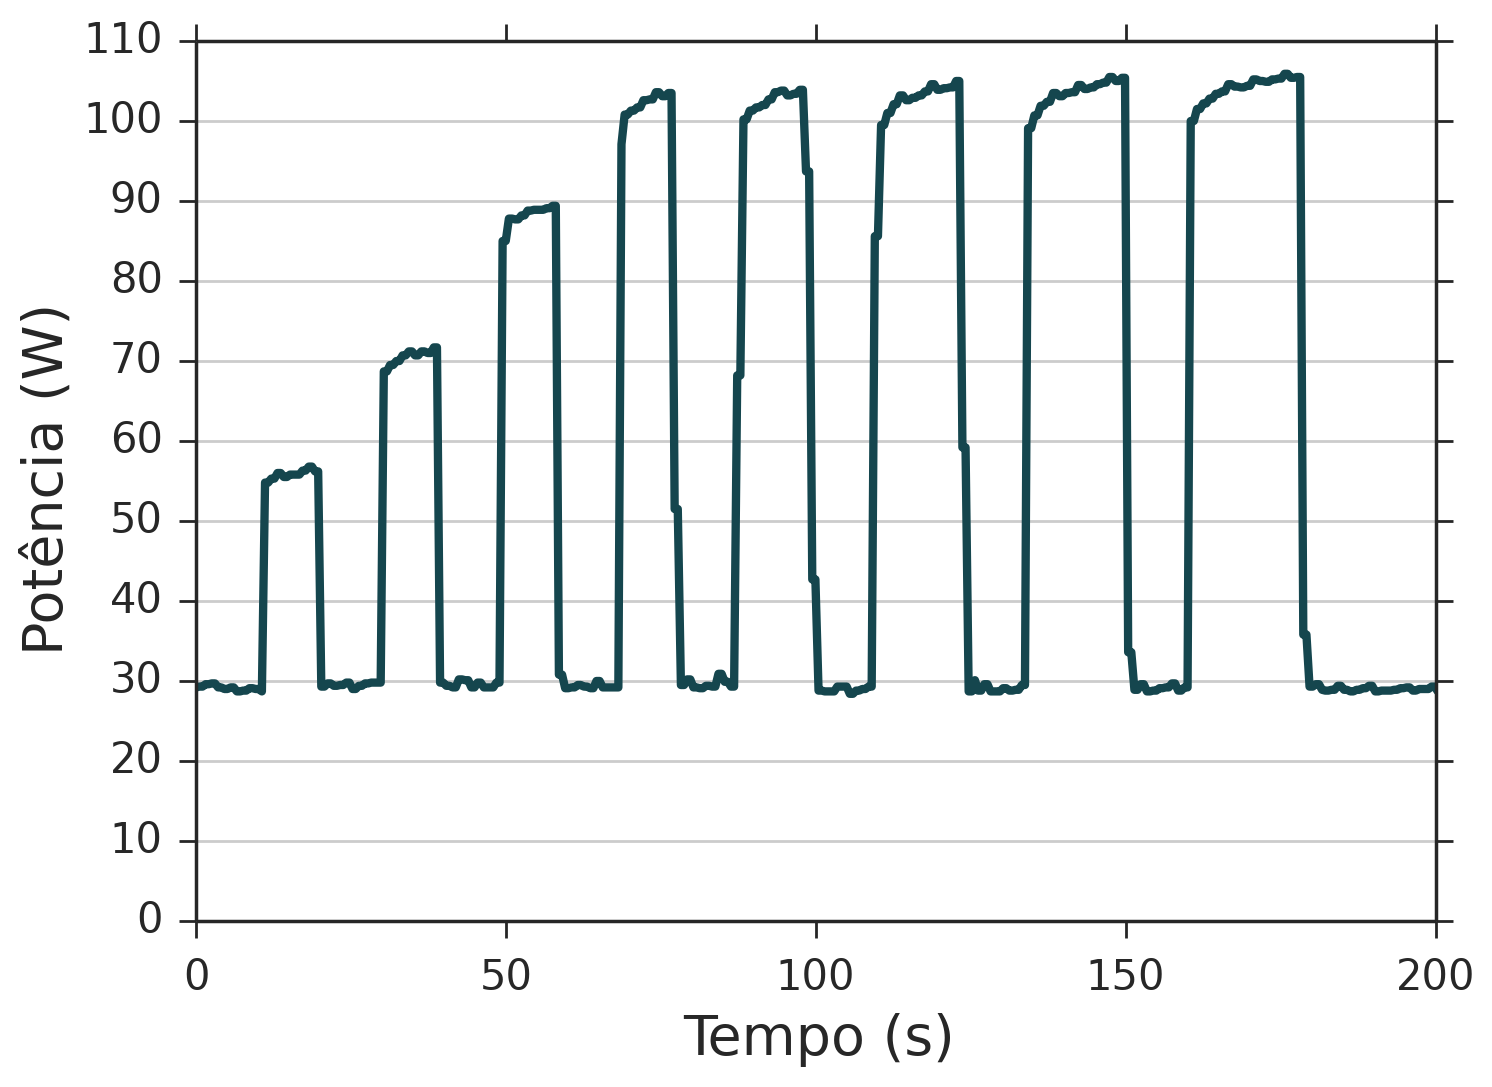
\includegraphics[scale=0.7]{figuras/MetMed/powerdump_var_workload.png}
\caption{Consumo de potência obtido pela biblioteca para execuções paralelas de uma aplicação}
\label{powerdump_pidigits}
\end{figure}\FloatBarrier

E como a CPU da máquina possui 4 núcleos, estes resultados não surpreendem.


\section{Medindo o consumo de aplicações}
\mbox{}

Usando a biblioteca descrita anteriormente, criamos uma simples ferramenta chamada {\tt energyanalyser}. Esta ferramenta roda várias vezes uma aplicação com seus argumentos e calcula seu consumo médio de potência, energia, dentre outras informações de consumo.

Para calcular o consumo de uma aplicação, a ferramenta começa a execução com uma medição do consumo total, sem a execução do comando, por um intervalo longo para a CPU (em torno de 10 segundos). Tendo calculado este consumo como base, ao final este consumo é desconsiderado da medição.

Escrita em C, roda em linha de comando e recebe os argumentos:

\begin{itemize}
\item Formato de saída, que pode ser {\tt h}, indicando que deve ser legível para uma pessoa, ou {\tt d}, indicando que deve permitir fácil extração de informações para um programa analisar (ex. gerador de gráficos). 

\item Número de vezes que o comando passado pelo usuário será rodado para ter seu consumo energético médio calculado.

\item Comando sobre o qual o usuário pretende fazer as medições.

\end{itemize}
Um exemplo de sua execução é dado abaixo:
\begin{figure}[htp]
\centering
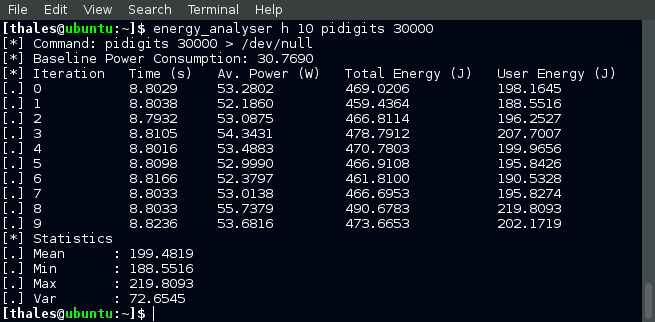
\includegraphics[scale=0.50]{figuras/MetMed/energy_analyser_pidigits.png}
\caption{Exemplo de execução do \emph{energyanalyser}}
\label{energyanalyser_pidigits}
\end{figure}
\FloatBarrier

